% 08-rui-ro.tex — Chương 8: Đánh giá và quản lý rủi ro

\chapter{Đánh giá và quản lý rủi ro}\label{ch:ruiro}

\begin{tomtat}[Nội dung chương]
Báo cáo liệt kê các rủi ro chính khi áp dụng sáng kiến, mức độ ảnh hưởng và biện pháp kiểm soát. Phần \emph{biện pháp} chủ yếu căn cứ các cơ chế đã có trong hệ thống;
phần \emph{đánh giá mức độ} là nhận định sơ bộ của nhóm biên soạn, cần được rà soát lại.
\end{tomtat}

\section{Bảng đăng ký rủi ro}

{\tablefont
\begin{longtable}{@{}L{0.9cm}L{3.5cm}L{1.5cm}L{1.5cm}>{\raggedright\arraybackslash}p{6.96cm}@{}}
\caption{Các rủi ro chính và biện pháp kiểm soát}\label{tab:rr}\\
\toprule
\hdrrow\hh{Mã} & \hh{Rủi ro} & \hh{Xác suất} & \hh{Tác động} & \hh{Biện pháp kiểm soát}\\
\midrule
\endfirsthead
\toprule
\hdrrow\hh{Mã} & \hh{Rủi ro} & \hh{Xác suất} & \hh{Tác động} & \hh{Biện pháp kiểm soát}\\
\midrule
\endhead
\bottomrule
\endfoot
R1 & Nhãn thực tế còn ít (khoảng 1.501 dòng), nhãn theo quy tắc có thể nhiễu & TB & Cao & Ưu tiên tuyệt đối nhãn thực tế; quy tắc nghiệp vụ bổ sung có kiểm soát tỷ lệ; đội chăm sóc ghi nhận kết quả để mở rộng nhãn; nghiên cứu làm mịn nhãn (Mục~\ref{sec:lamminh}).\\
\rowa R2 & Dữ liệu nguồn thay đổi cấu trúc, chậm hoặc thiếu tháng & TB & Cao & Chuẩn hóa cấu trúc khi nạp; kiểm tra độ mới và đầy đủ; nhật ký nạp; đề xuất ``hợp đồng dữ liệu'' với đội kỹ thuật dữ liệu.\\
R3 & Hành vi khách hàng thay đổi, mô hình lạc hậu & TB & TB & Huấn luyện lại định kỳ; giám sát độ lệch dữ liệu và điểm số; cổng xét duyệt trước khi thay mô hình.\\
\rowa R4 & Cảnh báo nhầm nhiều, đội chăm sóc quá tải & TB & TB & Giới hạn danh sách ở top 5\%; theo dõi độ chính xác trong top; đặt ngưỡng tải công việc; điều chỉnh tỷ lệ cắt khi cần.\\
R5 & Đội chăm sóc không hành động theo danh sách hoặc không ghi nhận kết quả & TB & Cao & Quy trình sử dụng danh sách; kịch bản chăm sóc theo lý do; chỉ tiêu tỷ lệ liên hệ; lãnh đạo bảo trợ; thử nghiệm đối chứng để chứng minh giá trị.\\
\rowa R6 & Gán nhầm khách mùa vụ, khách phục hồi, khách mới là rời bỏ & Thấp & TB & Đã loại các nhóm này khỏi phạm vi chính; bổ sung chỉ số mùa vụ và nhóm theo dõi riêng trong lộ trình.\\
R7 & Hiểu nhầm giữa xác suất, thứ hạng và tỷ lệ rời bỏ & Cao & Thấp & Đã ghi chú rõ trong tài liệu bàn giao; đề xuất đổi tên cột đầu ra; đào tạo người dùng.\\
\rowa R8 & Lộ hoặc dùng sai dữ liệu khách hàng khi mở rộng người dùng & Thấp & Cao & Mã hóa định danh; quản lý thông tin kết nối ngoài mã nguồn; thiết kế phân quyền theo cấp trước khi mở rộng; không lưu dữ liệu nhạy cảm vào nơi chia sẻ.\\
R9 & Phụ thuộc vào số ít người nắm hệ thống & TB & TB & Tài liệu bàn giao đầy đủ; đóng gói container; chuẩn hóa lệnh vận hành; đào tạo thêm nhân sự.\\
\rowa R10 & Sự cố máy chủ hoặc tràn dung lượng lưu trữ & Thấp & TB & Dọn dẹp theo quý; đóng gói phiên bản để khôi phục; mô hình cũ tiếp tục phục vụ khi huấn luyện mới lỗi.\\
R11 & Đánh giá quá lạc quan do ``nhìn trộm'' tương lai & Thấp & Cao & Chia dữ liệu theo thời gian có khoảng đệm; giữ bài thi cuối kỳ; kiểm tra lại trong quá khứ; so sánh với mô hình tham chiếu.\\
\end{longtable}}
\vspace{4pt}

\section{Ma trận rủi ro}

\begin{figure}[!ht]
\centering
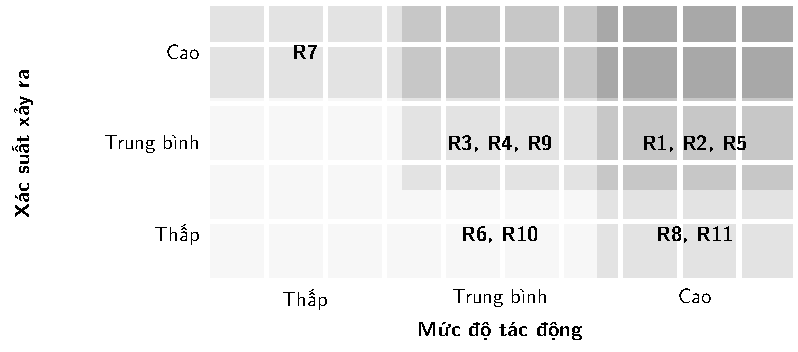
\includegraphics[width=383.2bp]{figures/fig10.pdf}
\caption{Ma trận rủi ro sơ bộ do nhóm biên soạn đánh giá}\label{fig:maTran}
\end{figure}

Ba rủi ro nằm ở ô trung bình--cao (R1, R2, R5) cần được theo dõi \textbf{hằng tháng} bởi lãnh đạo bảo trợ: chất lượng nhãn, độ ổn định của dữ liệu nguồn, và mức độ đội chăm sóc thực sự hành động theo danh sách.

\section{Nguyên tắc ứng phó khi có sự cố}

\begin{enumerate}
  \item \textbf{Dữ liệu lỗi hoặc đến muộn:} hệ thống ghi nhận trạng thái và không tự thay mô hình; danh sách vẫn xuất từ mô hình đã được xét duyệt; người vận hành kiểm tra nhật ký, yêu cầu kỹ thuật dữ liệu bổ sung.
  \item \textbf{Mô hình mới kém hơn:} bị từ chối tự động, mô hình cũ giữ nguyên; nhóm tác giả phân tích nguyên nhân.
  \item \textbf{Danh sách bất thường:} đối chiếu bảng giám sát điểm số; tạm ngừng chuyển danh sách cho nghiệp vụ nếu nghi ngờ.
  \item \textbf{Sự cố hạ tầng:} khôi phục từ phiên bản đóng gói gần nhất; chạy lại luồng công việc theo thứ tự.
\end{enumerate}
